\documentclass{standalone}

\usepackage{tikz, tkz-euclide}
\usetkzobj{all}

\begin{document}
	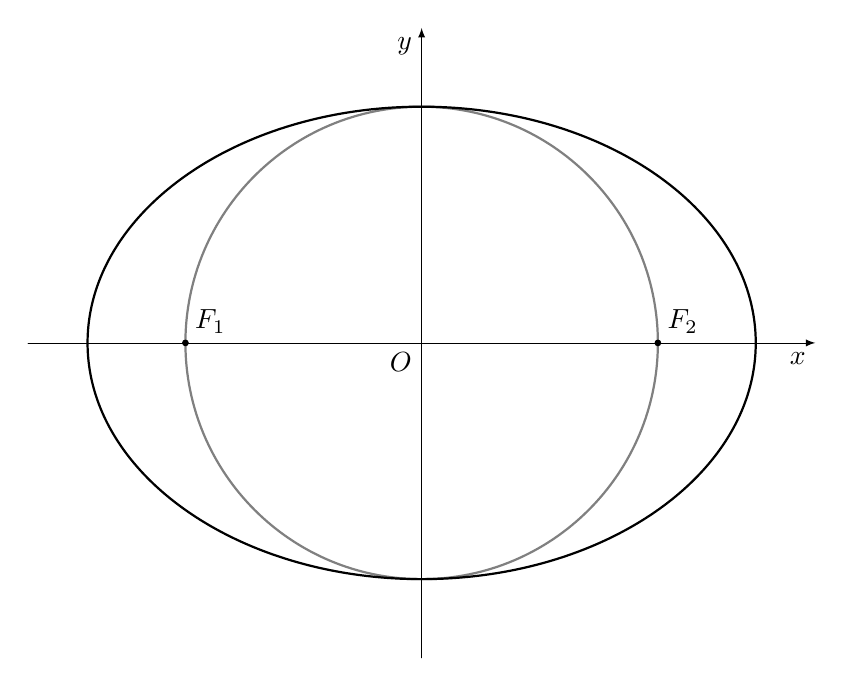
\begin{tikzpicture}
	\tkzDefPoints{0/0/O, 3/0/F2, -3/0/F1, -5/0/X1, 5/0/X2, 0/-4/Y1, 0/4/Y2}
	
	\tkzDrawCircle[thick](O,F2)
	
	\draw[thick] (O) ellipse (4.243cm and 3cm);
	
	\tkzDrawSegments[->, >=latex](X1,X2 Y1,Y2)
	\tkzDrawPoints[fill=black, color=black](F1,F2)
	\tkzLabelPoint[below left](O){\(O\)}
	\tkzLabelPoint[above right](F1){\(F_1\)}
	\tkzLabelPoint[above right](F2){\(F_2\)}
	\tkzLabelPoint[below left](X2){\(x\)}
	\tkzLabelPoint[below left](Y2){\(y\)}
	\end{tikzpicture}
\end{document}